\section{Inputs and outputs of a Lambert's solver computer algorithm}

At the very first section of Chapter 2, see \ref{sec:statement}, the statement
of Lambert's problem. However we only discussed it from the mathematical point
of view and not from a computational one. In this section, the input and output
parameters that any Lambert's solver algorithm must accept and return are
exposed and justified.

\subsection{Input parameters}

The input parameters of a solver are all the variables which the algorithm
requires in order to perform the computation. Among these parameters we can find
the following ones:

\begin{itemize}
  \item \textbf{Gravitational parameter $\mu$}: equivalent to $MG$, that is the
        mass of the attracting body time the gravitational constant. It can be
        understood as the strength of the Newtonian gravity field created by the
        attractor. It is a floating value.
  \item \textbf{Initial position vector $\vec{r_1}$}: the first observation vector
        as seen from an attractor centered inertial frame. Modern computers deal
        with vector representation in the form of pointers, lists or arrays.
        Three components are required, as the problem belongs to $\Re^3$.
  \item \textbf{Final position vector $\vec{r_2}$}: the second observation vector,
        as seen from an attractor centered inertial frame too. Similarly to the
        initial vector, three components are required.
  \item \textbf{Time of flight \textit{$\Delta t$}}: the time of flight between the
        initial and final position vectors. Should be of the type
        \textit{float}.
  \item \textbf{Number of revolutions $M$}: if the direct transfer is desired, the
        value of $M=0$ while for the multi-revolution scenario, the minimum
        number of revolutions is given by $M\geq1$. Therefore, this parameter
        only accepts \textit{integer} types.
  \item \textbf{Sense of motion}: this boolean\footnote{Boolean parameters only
          have two possible values: \textit{True} or \textit{False}.} parameter
        indicates if the orbit is prograde or retrograde so the proper normal
        vector to orbital plane can be identified together with the transfer
        angle. It is advisable to name this parameter as \textit{is\_prograde}
        so the user is aware of its boolean nature.
  \item \textbf{Type of path}: when dealing with the multi-revolution case, when a
        solution is found, two possible paths exist. Authors such us
        \cite{sun1977} usually refer to
        these two paths as \textit{lower} or \textit{higher} one. Similarly to
        the sense of motion, this is a boolean variable used to filter out the
        solution. The advice is to name this variable \textit{is\_low}.
  \item \textbf{Maximum number of iterations}: if exceeded, the algorithm did
        not converged to desired tolerance or simply diverged. This parameter
        is of the \textit{integer} type.
  \item \textbf{Absolute tolerance}: this floating value is used to check if the
        free-parameter value computed after a given iteration is within the
        expected limits.
  \item \textbf{Relative tolerance}: due to floating point errors, a relative
        tolerance is required to properly identify if the solution is within
        the expected limits of error, see \cite{randomascii2012} and
        \cite{christer2008}.
\end{itemize}

\subsection{Output parameters}

Regarding the outputs of a computer solver, only a pair of vectors are expected,
being each one the initial and final velocity ones.

\begin{itemize}
  \item \textbf{Initial velocity vector $\vec{v_1}$:} it is used to define the orbit
        together with the initial position vector. Again, a pointer, array or
        list must be used to store its components.
  \item \textbf{Final velocity vector $\vec{v_2}$:} it is useful for rendezvous applications
        and checking that the orbit holds both the final position and this one
        after being propagated the time of flight.
\end{itemize}

Figure \ref{fig:lambert_solver_computer} a Lambert's algorithm is being executed
with all the previously presented input parameters. The name for the routine is
composed by the solver's author and the year of publication.

\begin{figure}[h]
  \centering
  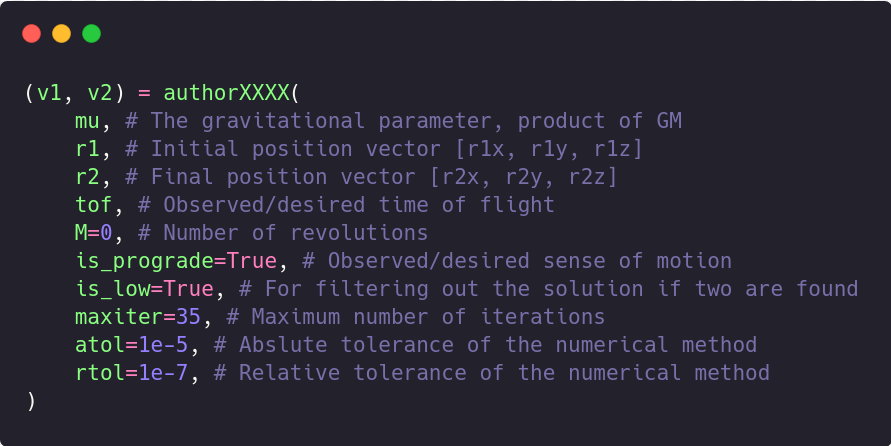
\includegraphics[width=\linewidth]{static/lambert_solver.png}
  \caption{A terminal emulator showing the execution of a Lambert's problem solver.}
  \label{fig:lambert_solver_computer}
\end{figure}


\subsection{Note on the usage of units in computer programs}

In the orbital mechanics and astrodynamics subjects it is advisable to make use
of quantities with the same characteristic order of magnitude in order to avoid
integration problems. However, there is a better approach: use canonical
formulae of the problem. By doing so, every problem can be translated to a
common space in which no units are required to perform the iteration workload.
Only in the last final step, the computed solution values are translated into
the original problem space. This reduces the propagation of errors during the
computation. Reader is encouraged to refer to \cite{wiesel2010}, who devotes a
section to this topic in his book about modern astrodynamics.

Another option is to let the user to manage the units. For example, if the
gravitational parameter $\mu$ has [km3/s2], the input values for the position
vectors $\vec{r_1}$ and $\vec{r_2}$ should be in [km] and the time of flight
$\Delta t$ in [s]. These input quantities will return the velocity vectors
$\vec{v_1}$ and $\vec{v_2}$ in [km/s], a common unit used for maneuvering
speeds.
